\documentclass[times]{cpeauth}

\usepackage{moreverb}
\usepackage{url}

\usepackage[dvips,colorlinks,bookmarksopen,bookmarksnumbered,citecolor=red,urlcolor=red]{hyperref}

\newcommand\BibTeX{{\rmfamily B\kern-.05em \textsc{i\kern-.025em b}\kern-.08em
T\kern-.1667em\lower.7ex\hbox{E}\kern-.125emX}}

\def\volumeyear{2010}

\begin{document}

\runningheads{A.~N.~Other}{A demonstration of the \journalabb\
class file}

\sloppy %gets rid of word overrun in some columns

\title{Lightweight Scheduling for the PRAGMA Cloud Testbed} 

\author{Shava Smallen\affil{1}\corrauth, Nadya Williams\affil{1}, Philip Papadopoulos\affil{1}}

\address{\affilnum{1}San Diego Supercomputer Center\break
University of California San Diego, 9500 Gilman Drive, La Jolla, CA 92093}\break

\corraddr{University of California San Diego, 9500 Gilman Drive, La Jolla, CA 92093. E-mail: ssmallen@sdsc.edu}

\begin{abstract}
The Pacific Rim Application and Grid Middleware Assembly (PRAGMA) is a community of research scientists and institutions from around the Pacific Rim that work together to enable scientific expeditions in areas such as biodiversity distribution and lake ecology.  PRAGMA's members collaborate on a testbed infrastructure and over the past four years, the technology focus has shifted to cloud and software defined networking as enabling technologies.  This short paper describes the design of a web-based cloud scheduler reservation system that will enable users to easily run and manage virtual clusters for their science.  Based on a client-server architecture, the cloud scheduler was designed so that it requires minimal installation and and management effort for participating PRAGMA testbed sites.   The PRAGMA cloud scheduler is built using a web-based room reservation tool called Booked and leverages several PRAGMA technologies such as pragma\_boot, Personal Cloud Controller,  and virtual network overlays (e.g., IPOP, ViNe).  We discuss our implementation of the pilot cloud scheduler and then describe future work.   
%add contribute and leverage shared resources
\end{abstract}

\keywords{Cloud, Scheduling, Resource Sharing, Virtualization} % NOT required for Proceedings

\maketitle

\vspace{-6pt}


% A category with the (minimum) three required fields
%\category{H.4}{Information Systems Applications}{Miscellaneous}
%A category including the fourth, optional field follows...
%\category{D.2.8}{Software Engineering}{Metrics}[complexity measures, performance measures]

%terms{Cloud, Scheduling, Resource Sharing}


\section{Introduction}
\label{Sec:intro}

The Pacific Rim Application and Grid Middleware Assembly (PRAGMA) researchers actively collaborate to enable scientific expeditions in areas of computational chemistry, telescience, biodiversity, and lake ecology~\cite{pragmaWeb}.  Founded in 2002, PRAGMA originally sought to advance the use of grid technologies for applications among a community of investigators working with leading institution sites around the Pacific Rim~\cite{pragmaReport2004}.  This included the deployment of a shared PRAGMA Grid testbed where participating sites could contribute and use resources as needed to develop and test new middleware and to conduct scientific experiments.  Testbed sites needed to install at a minimum the Globus toolkit~\cite{globus}, a local HPC job scheduler as well as other optional software such as MPICH-G2~\cite{mpichg2} and Ninf-G~\cite{ninfg}.  In November 2006, nineteen sites in thirteen countries were part of the testbed.  By 2009, the testbed had grown to twenty-seven sites in fifteen countries with a total of 1008 CPUs, more than 1.3 terabytes of memory, and over 24.7 terabytes of online storage.  However, as of 2011, the number of sites started to decline and maintaining the numerous and complex middleware and scientific applications at each local site required significant people effort and expertise.  Since PRAGMA participants often have varying levels of of funding, staff, and expertise, PRAGMA started to shift away from grid towards cloud technologies to simplify the infrastructure and to lower the amount of effort any site would need to participate in the testbed.  

The first phase of the PRAGMA cloud testbed started with three sites and focused around the creation of application-specific virtual machines and making them portable to  different cloud hosting environments like Rocks~\cite{rocks}, OpenNebula~\cite{opennebula}, and Eucalyptus~\cite{eucalyptus}.
One early example in 2011 was an AutoDock virtual cluster created for the Avian Flu Grid research team~\cite{pragmaReport2011}.   By 2012, the cloud testbed had ten sites with a total of 367 CPUs, 2.5 terabytes of memory and 657 terabytes of online storage.  To make it easier for users to assemble a multi-node virtual environment for running their scientific experiments, PRAGMA shifted its  focus in 2013 to the creation and management of virtual clusters.  The following technologies have been explored to facilitate the operation and use of virtual clusters on the PRAGMA cloud testbed.

% Decide to capitalize first word since http://www.quickanddirtytips.com/education/grammar/formatting-vertical-lists?page=2 indicates it's easier to capitalize
\textbf{Pragma\_boot:}  Rather than require a single cloud system at all sites, PRAGMA encourages sites to  deploy any virtualization technology that best fits their expertise. However, enabling a virtual cluster to be ported to different cloud hosting environments is a complex problem and requires tooling to retain the cluster relationship between head and worker nodes as well as software configurations.  In 2013, three pilot sites (UCSD, AIST, NCHC) developed a script to automate virtual cluster porting and demonstrated the same virtual cluster image being booted in three different cloud hosting environments, including Rocks/Xen, OpenNebula/KVM, and Amazon EC2.  Based on these experiences, the original prototype was redesigned and reimplemented as a \textit{pragma\_boot} toolkit with "drivers" to support  Rocks and OpenNebula.  In 2014, a feature was added to pragma\_boot to download and boot virtual cluster images from Amazon CloudFront~\cite{cloudfront}.

\textbf{Personal Cloud Controller:}  To provide researchers with an easy-to-use interface for managing the life cycle of their virtual clusters, a Personal Cloud Controller (PCC)  was started in 2014. This lightweight tool was designed to manage startup, status monitoring, and shutdown of a virtual cluster and was built on top of pragma\_boot and a well-known resource and workload management system HTCondor~\cite{condor}.   PCC also provided an option to create a multi-site virtual cluster leveraging an open-source virtual network overlay software IPOP~\cite{ipop} for creating its private network.  

\textbf{Software-Defined Networking}:   PRAGMA began investigating software-defined networking technologies such as OpenFlow~\cite{openflow} in 2013 as a way to create a private network among multi-site virtual clusters and to protect access to sensitive datasets.  PRAGMA then created the Experimental Network Testbed (PRAGMA-ENT) as a breakable, international testbed for use by PRAGMA researchers and collaborators.  In 2014, The PRAGMA-ENT team worked to create an reliable international Layer-2 connection with network engineers and developed AutoVFlow~\cite{autovflow} that can provision private virtual network slices for each application, user, and/or project~\cite{pragmaReport2014}.  

In late 2014 during the PRAGMA27 workshop, a lightweight scheduler was proposed to coordinate virtual hosts and clusters running on the different cloud deployments  and leveraging the above described technologies.  The next section discusses the general requirements of the cloud scheduler and Section~\ref{Sec:Design} discusses the design options that were considered.  The architecture of the cloud scheduler is provided in Section~\ref{Sec:Arch} and Section~\ref{Sec:Pilot} discusses our pilot implementation.  Section~\ref{Sec:Conclusions} concludes with our planned future work.  

% NOTES AND SNIPPET TEXT THAT WAS NO LONGER RELEVANT
%In 2012, a \textit{vm-deploy} script was developed to automate the process of launching a virtual machine from distributed Gfarm filesystem~\cite{gfarm) to an OpenNebula deployment.  , which later became \textit{pragma\_boot} in 2013, to automate the VM porting process from one cloud deployment to another~\cite{pragmaReport2012,pragmaReport2013}.  

%In Phase 2, PRAGMA started using Gfarm~\cite{gfarm} as a mechanism to distribute and migrate VMs to different sites~\cite{pragmaReport2012} and in Phase 3 grew the cloud testbed to ten sites in 2012 with a total of 367 CPUs, 2.5 terabytes of memory, and 657 terabytes of online storage.   To facilitate the creation of application VMs, a web-based, easy-to-use user interface was developed for the Ezilla tool~\cite{ezilla} so that users can drag-n-drop the applications they need into their own custom VM image~\cite{pragmaReport2013}.  

% 2005-2006: 19 sites in 13 countries, with a total of 662 CPUs, near- ly 1 terabyte of memory, and 7.3 terabytes of online storage.
% 2006-2007: The PRAGMA testbed grew from 19 sites in 13 countries to 26 sites in 14 countries, with a total of 726 CPUs, more than half a terabyte of memory, and 13.2 terabytes of online storage
% 2007-2008: During this last year, the PRAGMA grid grew from 26 sites in 14 countries/regions to 30 sites in 17 countries/regions, with a total of 1109 CPUs, more than one terabyte of memory, and 26.7 terabytes of online storage.
% 2008-2009: During the last year, the PRAGMA Grid has grown to 27 sites in 15 countries/regions with total of 1008 CPUs, more than 1.3 ter- abytes of memory, and over 24.7 terabytes of online storage.
% 2009-2010:  Currently, the PRAGMA Grid has 24 sites in 16 countries/regions which provides a total of 1022 CPUs, more than 1.3 terabytes of memory, and over 24.8 terabytes of online storage. 
% 2010-2011: Since PRAGMA 17 (October 2009, Hanoi), the Resources Working Group has decided to migrate from grid to cloud through experimentation with virtualization technologies
% 2011-2012: At PRAGMA 20 (March 2011, Hong Kong), the three pilot sites demonstrated this Phase 1 experiment and findings. These results have excited many PRAGMA sites and motivated them to join this effort. Since then, seven more sites have set up VM hosting services and migrated the three application VMs. These sites are: Indiana University (IU), ASTI, MIMOS, LZU, Osaka University, CNIC and University of Hyderabad (UoHyd).
% 2012-2013: Our progress in porting (a form of sharing) VM images has taken place in three phases. In the first phase, (completed in early 2011), we successfully demonstrated a manual port of three application VM images among three different VM hosting environments (i.e., a pairing of a VM hosting platform with VM hosting managing software, e.g. Open Nebula). Phase 2 began at PRAGMA 20 (March 2011, Hong Kong), where, based on what we learned from the phase 1 experiments, we designed a PRAGMA cloud infrastructure to use Gfarm for VM image depository and sharing and to automate VM deployment process on various virtualization platforms that make up the PRAGMA multi-cloud. At PRAGMA 21 (October 2011, Japan), we demonstrated the automated deployment of a GEO Grid VM image from Gfarm to three pilot sites?AIST, NCHC and UCSD.  After PRAGMA 21, we started Phase 3 of the VM sharing experiment with four objectives: 1) to expand PRAGMA cloud resources; 2) to enhance Gfarm functionality and performance; 3) to author and run more application VMs and 4) to develop an easy-to-use user interface for creating VM images.
% 2013-2014: 


\section{Scheduler Requirements}

PRAGMA had the following three key requirements for a cloud testbed scheduler to enable multiple users to access the resources at a  given time:

\textbf{Low participation overhead}:  One key requirement for the cloud testbed scheduler was that it had to be lightweight and required  minimal effort and minimal expertise for a site to add their cloud deployment to the list of resources available for scheduling.   Similarly, the scheduler would need to work across multiple cloud systems (e.g., Rocks, OpenNebula, and OpenStack~\cite{openstack}) so that sites do not have to learn and install additional cloud deployment tools. 

\textbf{Easy to use}:  Currently, to execute a virtual cluster on the PRAGMA cloud testbed, users needs to contact each site individually to gain access to their cloud deployment, upload their images, and launch their virtual cluster either using pragma\_boot  if it is available or manually via a sequence of defined steps.   The design of the PRAGMA cloud scheduler should first simplify this process by ensuring that pragma\_boot gets deployed more broadly and port it to more cloud systems as needed.   The scheduler should also provide a simple web interface for users to see the available resources and sites, construct their virtual cluster, and manage their images.

\textbf{Scale to tens of users:}  While the PRAGMA community was composed of nineteen active institution sites in 2014, the initial number of expected users for the cloud testbed is in the tens of users, not hundreds nor thousands.  Therefore, we can prioritize simplicity over scalability and give higher priority to the requirements of low participation overhead and ease of use.

\section{Scheduler Design}
\label{Sec:Design}

In our design discussions, we first looked at some existing solutions that might be adapted for PRAGMA's scheduling needs.  Open source batch schedulers like Slurm~\cite{slurm}, TORQUE~\cite{torque}, or HTCondor, are used to manage space shared resources.  There are also other testbeds like Grid'5000~\cite{grid5000},  GENI~\cite{geni}, and PlanetLab~\cite{planetlab} that have their own tools for using and managing their infrastructures. In general, we found these tools had different goals and were too heavy weight for PRAGMA.  Some tools were better documented than others but all had a fairly high learning curve and would have been non-trivial to adapt for PRAGMA's cloud testbed, which had a strong application and virtual cluster focus.

We next searched for a simpler approach to scheduling and found a number of open source web-based calendar reservation systems that seemed promising.  These systems were designed to manage meeting room reservations, hotel room reservations, or equipment rentals.   Their interfaces would be more familiar to users in their everyday lives and thus well suited to the different types of PRAGMA users.  In addition, several of these tools were significantly less complex than the batch and testbed scheduling tools above.  Later, we found a web-based calendar reservation system called GridPrems~\cite{gridprems} for Grid'5000 indicating a simpler interface was sometimes needed even for their users.

Some of the calendar reservation systems we looked at like Reservations~\cite{drupalreservations}, Merci~\cite{merci}, and Booking\_calendar~\cite{wordpressbooking} were plugins for Drupal~\cite{drupal} or Wordpress~\cite{wordpress}.  However, the majority of tools were PHP based with a relational database backend like the Meeting Room Booking System~\cite{mrbs}, Booked~\cite{booked}, and Classroombookings~\cite{classroombookings}.  For each system, we evaluated 1) how easy it would be to manage resources, reservations, and users as well as to add new parameters and features; 2) how intuitive the GUI interface was with respect to menus and navigation and if it had a clean, modern, and uncluttered look; 3)  how easy it was to install and setup a prototype instance. One deficiency that all systems had was that they only allowed one reservation per resource.

Booked~\cite{booked} from Twinkle Toes software seemed the best suited to our needs compare to all the calendar reservation systems we evaluated.  It was easy to setup, had  a good look and feel, and was customizable.  It also had some nice additional features like usage reporting, a REST API interface, LDAP and Active Directory support, fine grained roles and permissions management, and user and group quotas.  After working with Booked during our pilot setup, we did find some weaknesses.  First, the documentation was very sparse and any needed PHP changes were time consuming due to its heavily object-oriented structure (i.e., we had to go through many source code files to find the right place to change  or add functionality).   The granularity of Booked reservations is currently limited to an hourly basis and for today's PRAGMA needs this is sufficient because the time it takes to start up the virtual cluster 
is tens of minutes and  the user reservation is expected to  be on the order of days. The reservation granularity can be optimized in the future in order to avoid a potential of underutilized resources when the virtual cluster startup becomes minutes. 

\section{Scheduler Architecture}
\label{Sec:Arch}

One key requirement for our cloud scheduler was to enable users to create and manage virtual clusters on the PRAGMA cloud testbed with minimal effort. 
The basic workflow and steps for how a user would start a virtual cluster are summarized below:

\begin{enumerate}
\item A user does a general search for available resources based on the number of CPUs, memory size, and networking configuration (e.g., IPOP, ViNE~\cite{vine}, or PRAGMA-ENT) that is needed.  
\item Available resources that fit the criteria are displayed to the user and their availability is shown in a calendar layout.  
\item The user selects the subset of  desired resources, the timeframe, virtual cluster image, and configuration details and submits it to the Cloud scheduler.  Once the reservation is verified and confirmed, the user will get an email confirmation.  
\item When the reservation is ready to be activated, the cloud scheduler will use PCC and pragma\_boot to launch the virtual cluster, automatically configure the private and public network configuration on the virtual cluster nodes, and email the user when the reconfigured cluster is ready.   
\end{enumerate}

Figure~\ref{Fig:Flow} shows the above steps in a use case sequence diagram where \textit{PRAGMA Booking} refers to our customized Booked instance.  PCC will monitor the health of the virtual cluster and when the reservation is close to expiring, will notify the user via email. The user then has an option to extend the reservation if resources are available.  Otherwise, when the time expires or the user chooses to end the reservation, the virtual cluster will be shut down.

\begin{figure}[htbp]
\begin{center}
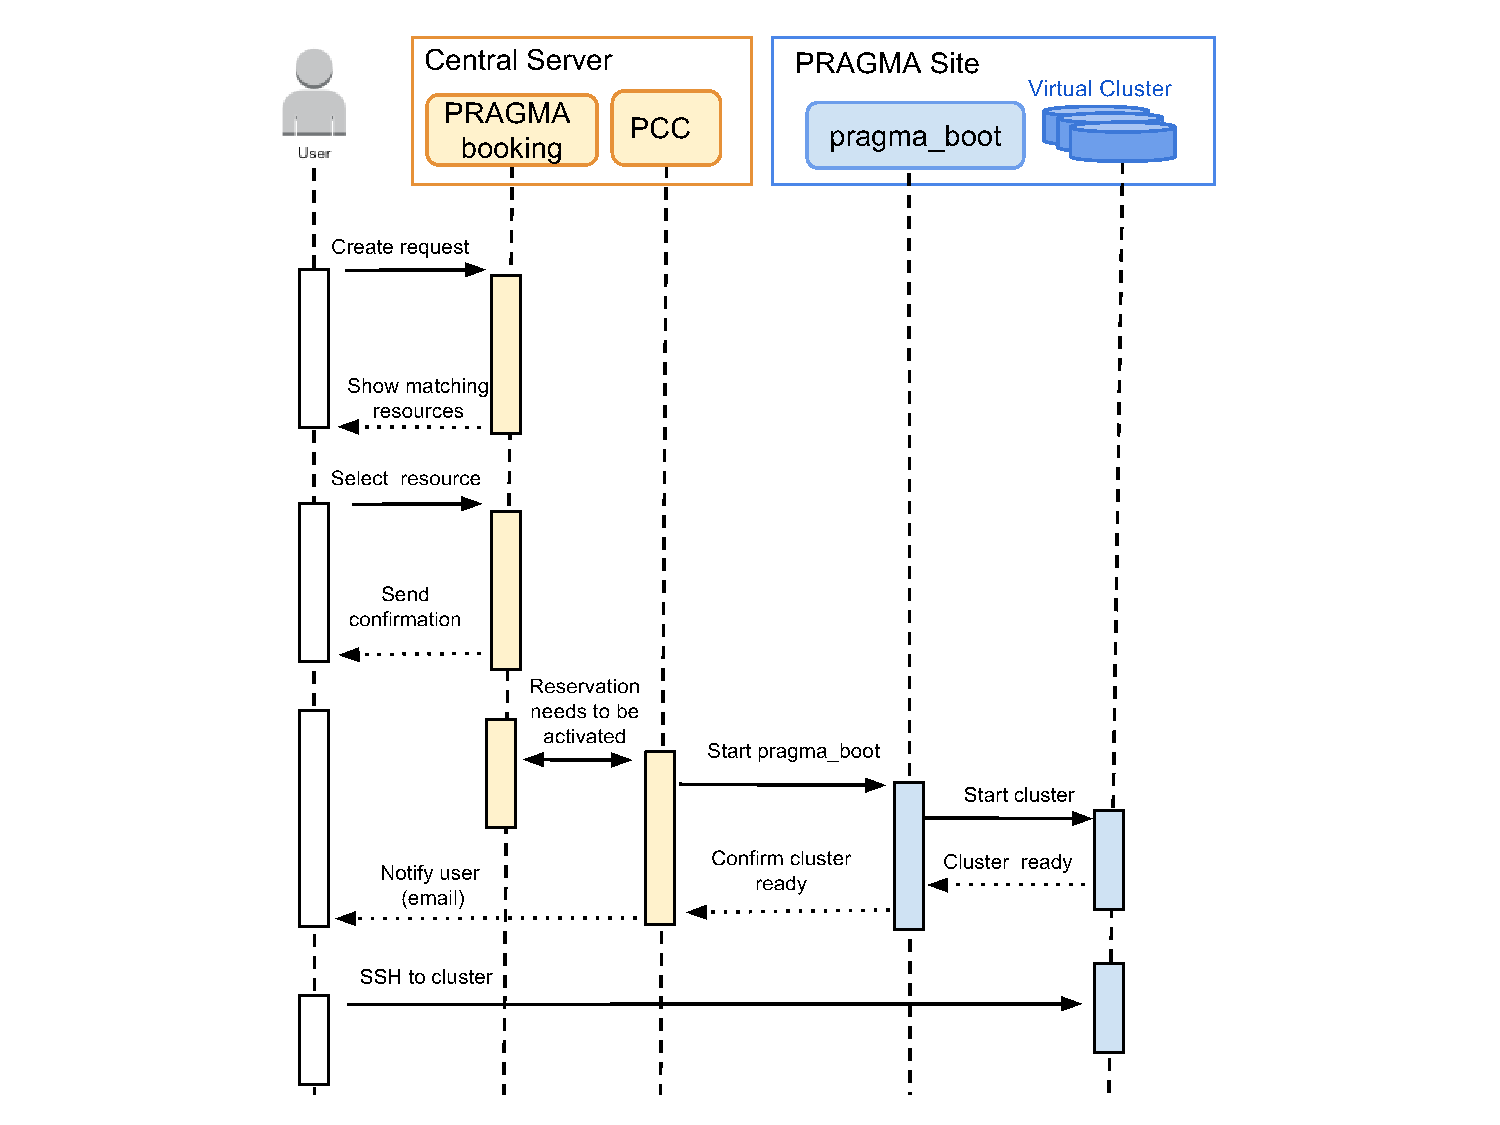
\includegraphics[width=\columnwidth]{figures/flow.ps}
\caption{The flow of a user request to start a virtual cluster and the components that are involved in the cloud scheduler.}
\label{Fig:Flow}
\end{center}
\end{figure}

The other key requirement for the cloud scheduler was that it should require minimal effort for PRAGMA sites to participate in the PRAGMA testbed.  Therefore, we opted for a simple client-server architecture, where the client is a small PRAGMA package that interfaces with a site's local cloud system.  Currently, the PRAGMA Package consists of an SSH service and pragma\_boot, which is a small Python package that can be installed via RPM and can be configured in less than an hour.  The server component is composed of the PRAGMA Booking interface and PCC, which gets launched for each user.  The architecture for the PRAGMA cloud scheduler is shown in Figure~\ref{Fig:Arch}.

\begin{figure}[htbp]
\begin{center}
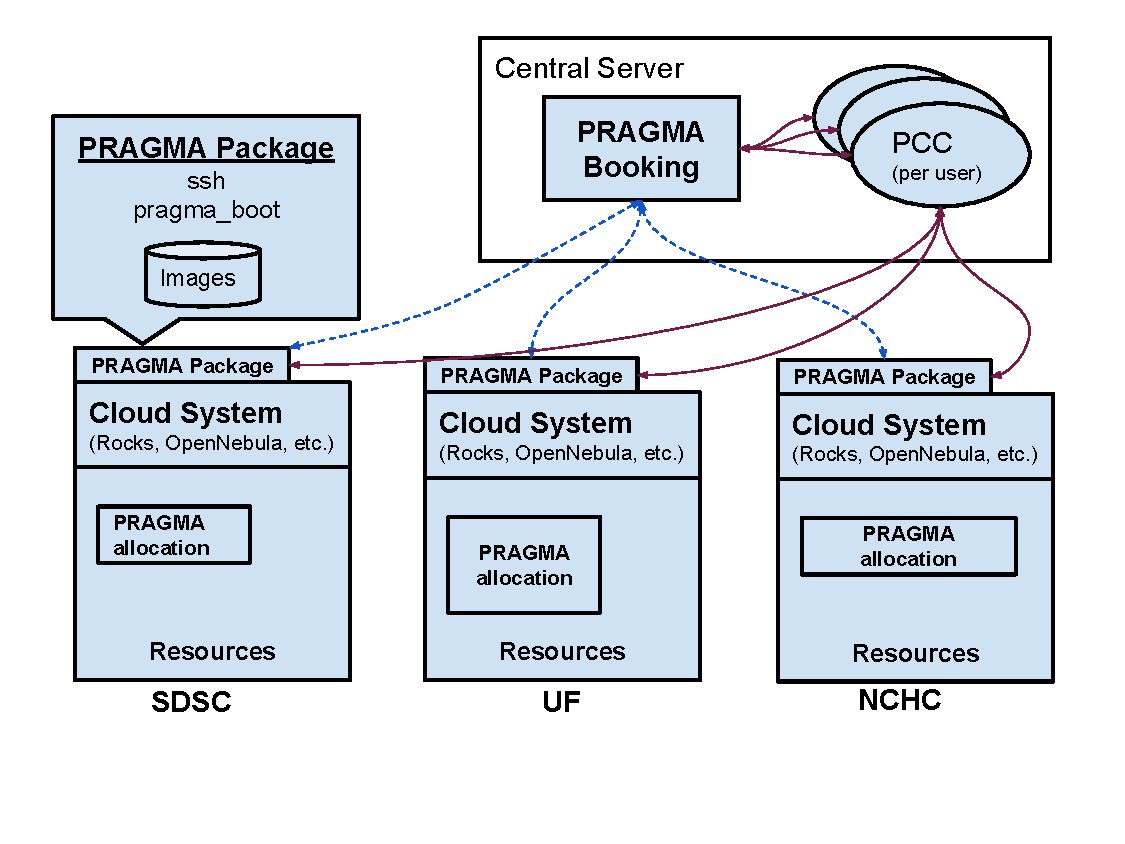
\includegraphics[width=.75\columnwidth]{figures/arch.ps}
\caption{Architecture for the PRAGMA cloud scheduler.}
\label{Fig:Arch}
\end{center}
\end{figure}

\section{Scheduler Pilot}
\label{Sec:Pilot}

In our pilot implementation of the cloud scheduler, we made a number of temporary assumptions to simplify the design.

\textbf{Virtual cluster images are already available at each site:}  For our pilot, we worked with a small number of virtual cluster images and pre-installed them to each cloud system so they were readily accessible by pragma\_boot.  We had the following three images: 1) a basic SGE Rocks virtual cluster; 2) an AutoDock virtual cluster;  3) a Lifemapper~\cite{lifemapper} compute virtual cluster.   

\textbf{Developed and used a PCC stub:}  Since PCC is also under active development and was not easy to install, we used a simple stub to substitute for its functionality.  The stub is a small Python script called \textit{pcc-check-reservations} that polls PRAGMA Booking via its REST interface and monitors reservations.  Once it finds a reservation that needs to be activated, it launches pragma\_boot via SSH.  It does not  monitor the virtual cluster nor does it email the users when their reservation are about to expire.  

\textbf{Only single site virtual clusters can be launched:}  So far, we have only experimented with multi-site virtual clusters using IPOP.  When virtual cluster images have been IPOP-enabled, IPOP and an automated configure script will assign private IP addresses to each node on boot.  For Rocks virtual clusters, there is a Rocks roll~\cite{ipoproll} that will automate the IPOP installation and install the configure scripts.  IPOP can be used by any PRAGMA site but some sites may have support for better performing network overlays created with ViNE or software-defined networking tools.  Therefore, our long-term goal is to automatically select the most appropriate network overlay depending on the virtual cluster specification and leave IPOP as the lowest common denominator or default.

Much of our work in this pilot focused on creating the PRAGMA Booking interface.  This required the following customizations to Booked:

\begin{itemize}
\item Added the ability to make multiple reservations on a resource per time slot to allow more than one virtual cluster to run simultaneously on a site.   This was the most extensive change we made to Booked.  Fortunately, no changes were needed to the backend database but it required several changes to the GUI code to allow an additional reservation to be made on a resource and to display multiple reservations per time slot in the calendar views.  In total, enhancements were made to seven PHP files and two template files.
\item Added a custom field for a public SSH key  to the user profile.  When PCC launches a virtual cluster, it will pull the public SSH key from the user's  profile and give it to pragma\_boot so that the user can login as root once the virtual cluster is launched.   The ability to use a root login is not required for all but can be needed in some case if users want to do system modifications. A user with a root login has a full ownership of the virtual cluster. 
\item Added custom fields for CPU count, amount of memory per host, and virtual cluster image name to the reservation specification.
\item Added custom fields for CPU count, amount of memory per host, site hostname, and ENT capability (enabled, disabled) to the resource specification.
\item Added a numeric count as a custom field type.  Booked only provided text matching on search so if a host had 16 CPUs available and the user requested 8 CPUs, the search would fail per "16" != "8" inequality.  By adding count as a custom field type, the search would do a numeric comparison on the values and the search would succeed for 8 <= 16.
\item Added custom reservation statuses: "Starting", "Running", and "Stopping".  Each reservation status is shown as a different color in  the calendar view.
\item Added the ability to retrieve and set the reservation status from the Booked REST API.  	
\item Added the PRAGMA logo to the header.
\end{itemize}

We also fixed the following bugs in Booked and plan to work with the developer to integrate them back into the distribution:

\begin{itemize}
\item Fixed bug that allowed users to make reservations for past time frames.
\item Fixed a time conversion bug that was preventing updates to existing reservations.
\item Fixed bug where the username was getting set to a blank value when a reservation was updated via the REST API. 
\item Fixed bug that would not recognize zero as a valid value (e.g., specifying a virtual cluster with just a frontend and 0 compute nodes).  
\end{itemize}

Some sample screenshots of the PRAGMA Booking user interface are shown in Figure~\ref{Fig:Booked}.  Likewise, Figure~\ref{Fig:Reports} shows some screenshots of the administrations options and usage reports.  We created a  Booked Rocks roll~\cite{cloudscheduler} which packages the software with our customizations and automates its installation and publishing of sample data.

\begin{figure*}[htbp] 
\begin{center}
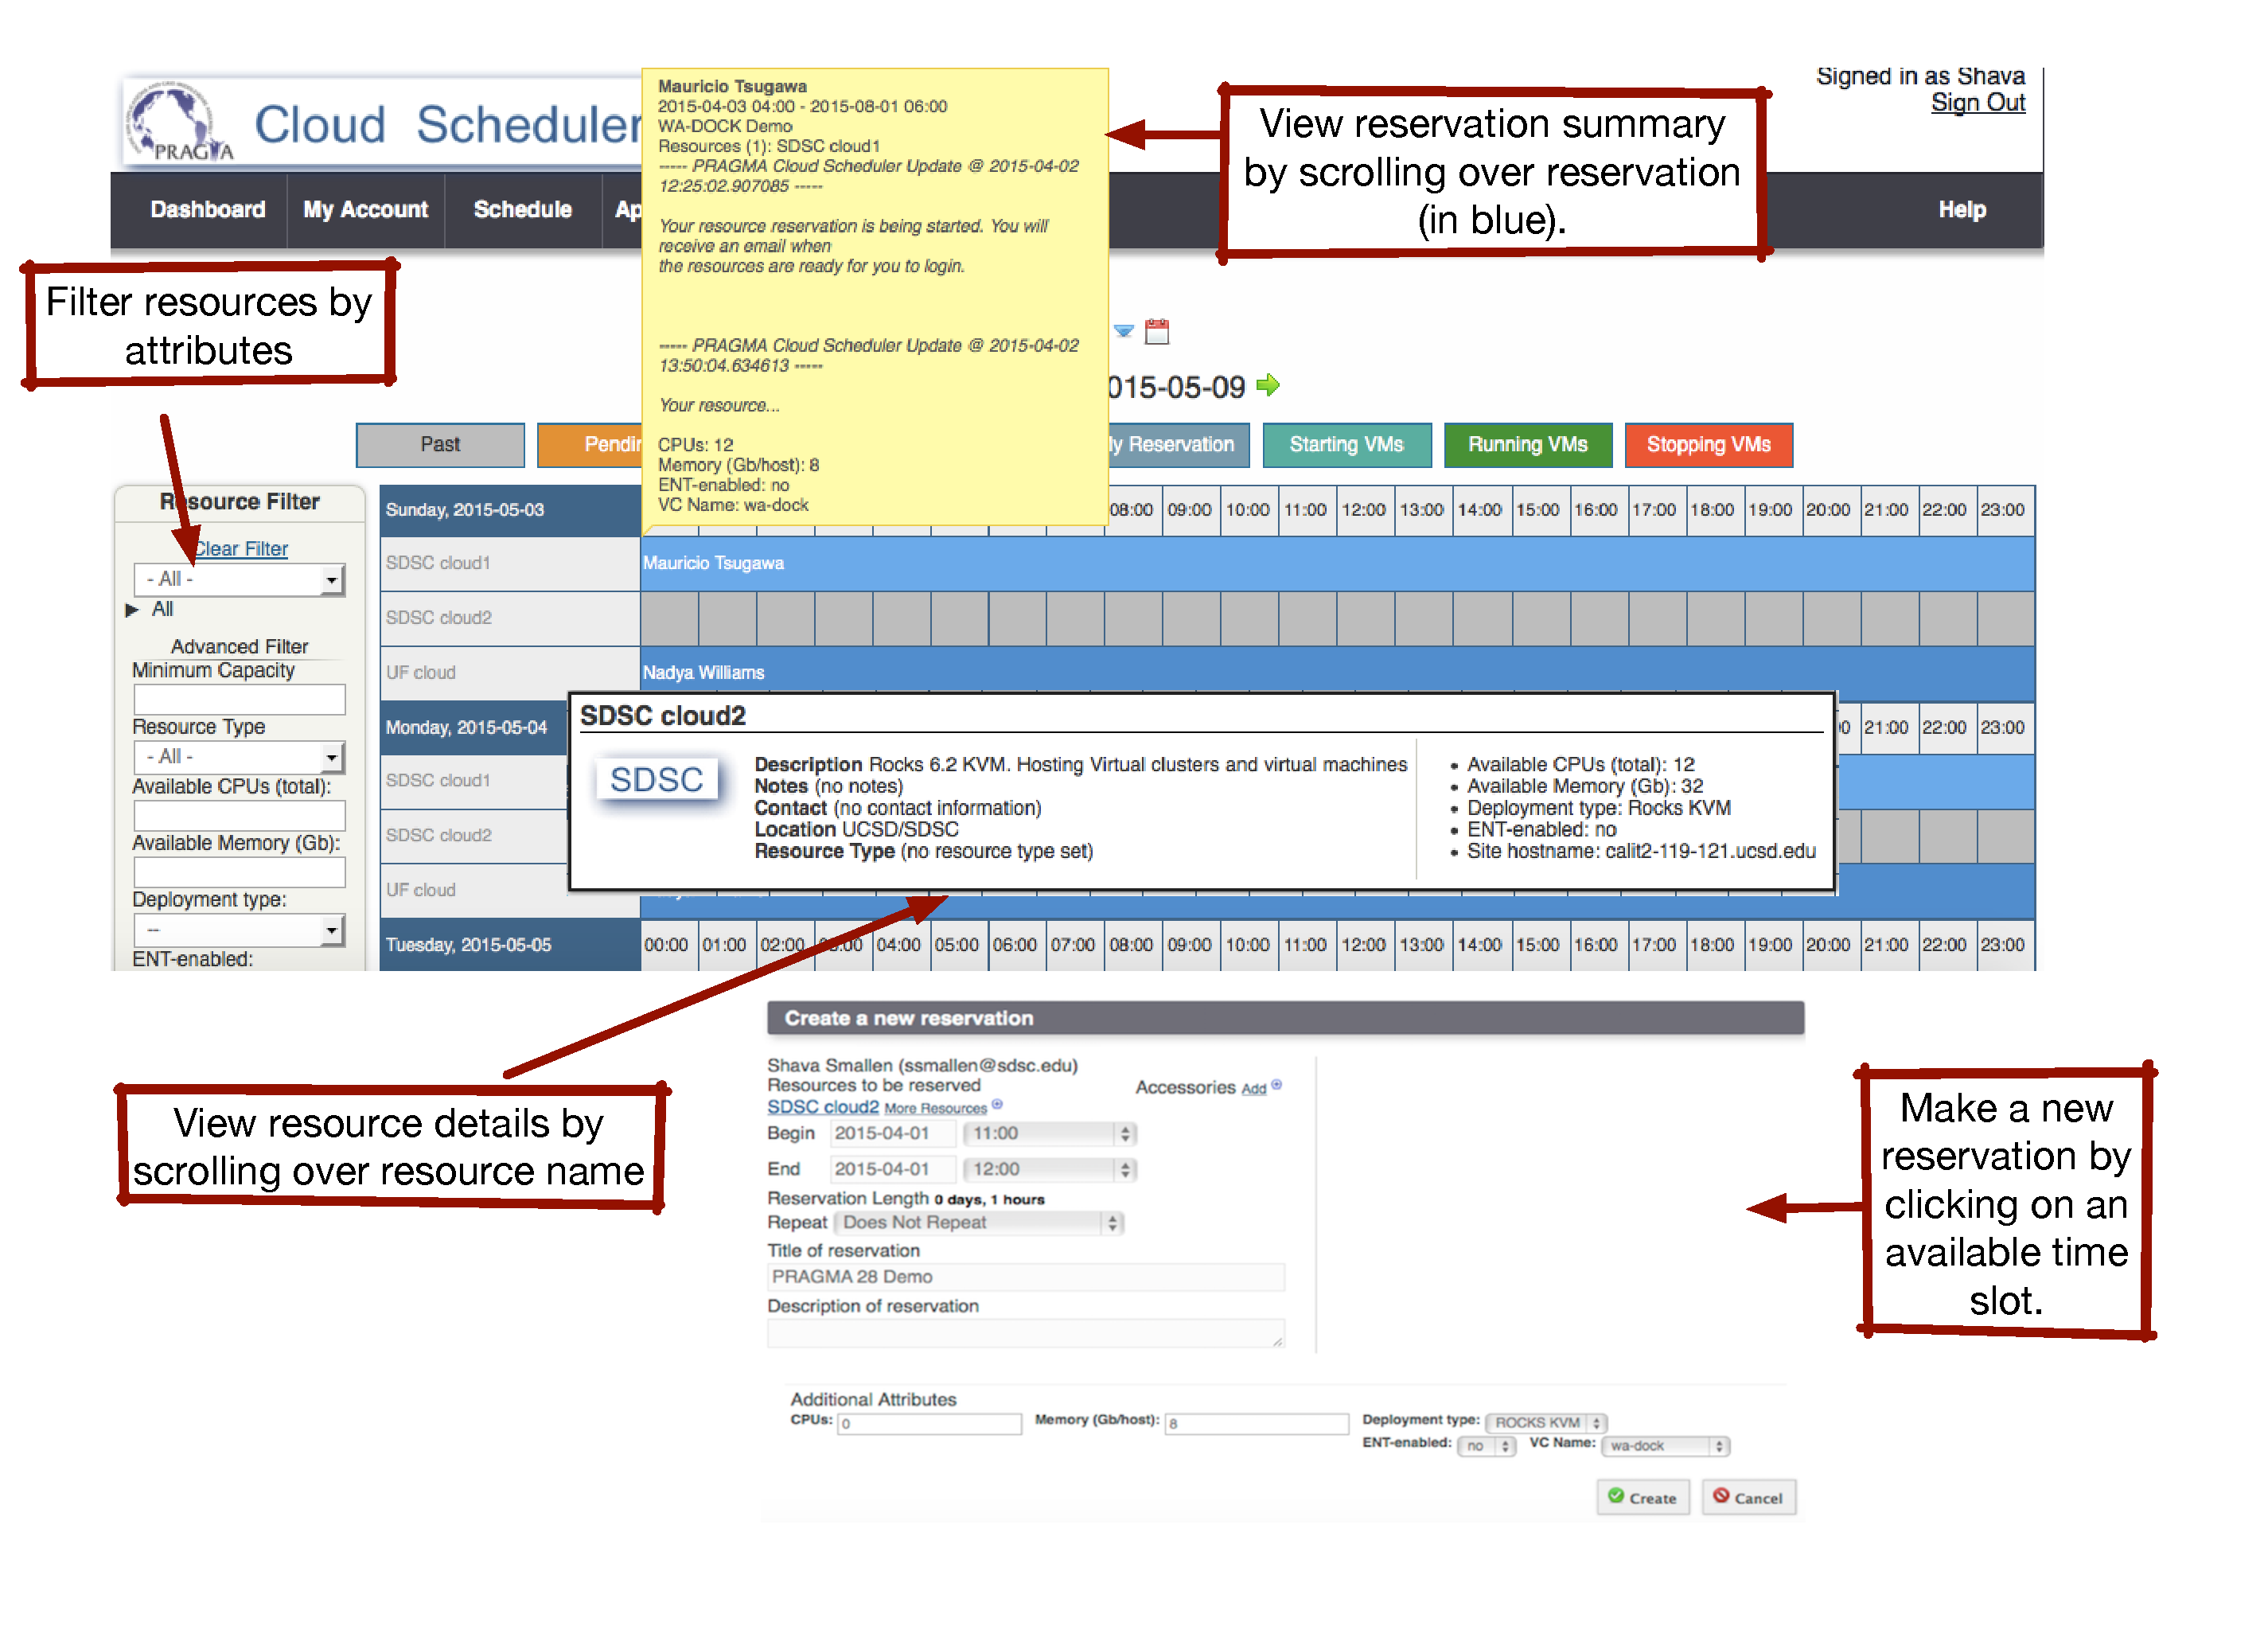
\includegraphics[width=\textwidth]{figures/bookedReservationScreenshot.eps}
\caption{Screenshots of the PRAGMA Booking user interface showing how a user can view and filter resources, view reservation summaries, and create a new reservation.}
\label{Fig:Booked}
\end{center}
\end{figure*}

\begin{figure*}[htbp]
\begin{center}
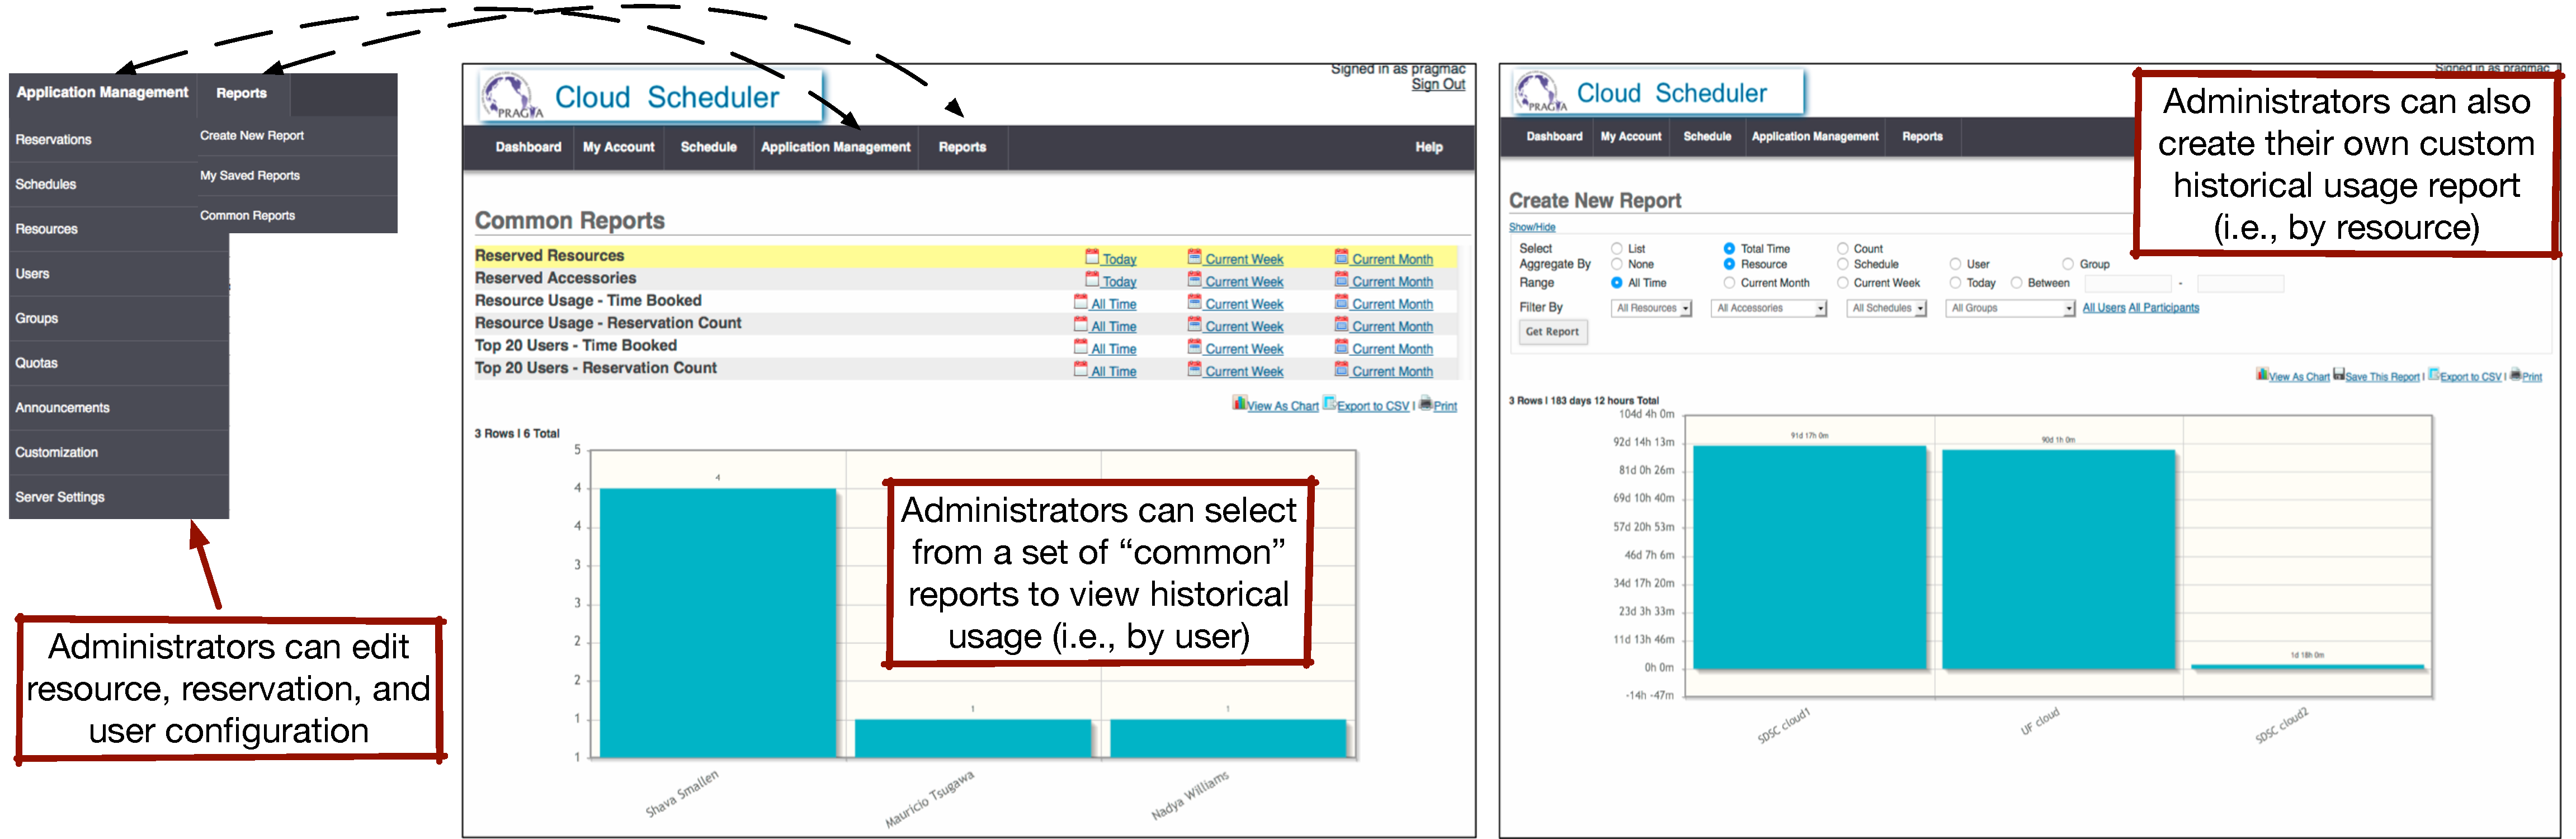
\includegraphics[width=\textwidth]{figures/bookedReportScreenshot.eps}
\caption{Screenshots of the PRAGMA Booking admin and reporting interface showing where an administrator can edit configuration details and then view usage reports.}
\label{Fig:Reports}
\end{center}
\end{figure*}

\section{Conclusions and Future Work}
\label{Sec:Conclusions}

This paper described the the design and pilot implementation of a  scheduler for the PRAGMA cloud testbed.  Since the scheduler does not need to scale beyond tens of users, we prioritized ease of use and low installation and maintenance overhead and opted for a simple client-server design.  The server has an intuitive web GUI frontend based on the Booked web reservation system software.  

In the pilot implementation of the cloud scheduler  we made a lot of temporary assumptions, and  our future work will address them.  We will first work on integrating IPOP and PRAGMA-ENT into the cloud scheduler.  Next, we will rework the PCC software and integrate HTCondor so it's used in personal mode allowing us to keep a light footprint on each of the PRAGMA sites.  Finally, we will investigate using the CloudFront option in pragma\_boot to manage application virtual cluster images and staging them to each of the sites.     We will package and document the resulting software so that new users and sites can get quickly onto the PRAGMA cloud testbed and use it as an experimental service to test new science and infrastructure tools.


%ACKNOWLEDGMENTS are optional
\section{Acknowledgments}

The authors would like to thank Jose Fortes and Mauricio Tsugawa for their help during our initial design discussions and for providing resources at University of Florida during development.

\bibliographystyle{abbrv}
\bibliography{paper}  

\end{document}

